\documentclass{article}
\usepackage[final]{nips_2018}
\usepackage[utf8]{inputenc}
\usepackage[T1]{fontenc}
\usepackage{hyperref}
\usepackage{url}
\usepackage{booktabs}
\usepackage{amsfonts}
\usepackage{nicefrac}
\usepackage{microtype}
\usepackage{gensymb}
\usepackage{graphicx}
\usepackage{subfig}
\usepackage{wrapfig}

\title{Learning to Grasp: From the Cornell Dataset}
%\author{George Maratos (need to mention advisor)}

\begin{document}
\maketitle

\begin{abstract}
Fully autonomous grasping is a difficult problem. In this project, I explored
the cornell grasping dataset and tried to see if I could build a model that
learning how to model the information from this. The task to be learned was
difficult, and the dataset was small, so I tried to mitigate these challenges
with pretraining.
\end{abstract}

\section{Introduction}
In the robotic grasping problem the goal is, given an object, select a grasp
configuration such that the object can be restrained and
manipulated to some desirable end. Finding such configurations is difficult
because of the multi-modal nature of the input and the fact that there can be
more than one suitable grasping location, leaving machines with the task
of determing optimality for predicted configurations.

Some of the earliest reviews of algorithms for grasping \cite{shimoga96,bicchi00},
shows that the premliminary work involved solving unconstrained linear programming
problems using objectives that measure dexterity and grasp quality. A grasp
algorithm in this context is one that is able to calculate the stability or
equilibrium of its grasp, and they are collectively refered too in the
review as \textit{robot grasp synthesis algorithms}.

The review by Sahbani \textit{et al.} \cite{sahbani12}, makes a distinction
between methods that model the kinematics and dynamics of a grasp, like the
synthesis algorithms, and methods that mimic human grasp strategies or learn
from data. The former called the analytic methods and the latter empirical.
They divide the analytical techniques into force closure methods and task
oriented. The authors determine that force closure is able to find stable
grasps but are usually not task oriented, and the task oriented strategies tend
to be computationally intensive. The empirical methods on the other hand can
model task oriented features, but struggle to generalize well to new objects.

Bohg \textit{et al.} \cite{bohg14} observe that grasping methods typically aim
to address the following object types: fully known, familiar, or fully unknown.
When considering the empirical methods, fully known represents objects that
have been seen in the training data before and the grasping problem reduces to
locating the object and applying a similar grasp to those from experience.
The familiar objects are assumed to have some matching characteristics to objects
from the training data, like shape, color, and texture. Familiar objects
introduce a new challenge of calculating similarity between objects so that
the appropriate grasp can be determined. On the other hand, grasping algorithms
will have no experience to utilize when approaching fully known objects. Methods
of this category typically rely on finding structures in the features to
synthesize a grasp.

The focus of this work is to build empirical models for grasp synthesis using
the Cornell Grasp Datset \cite{lenz15}, and evaluating them on familiar and
fully unknown objects. Section 2 will describe previous methods for grasp
synthesis. Section 3 will focus on analysis of the dataset and a description
of the task. Section 4 will contain the experimental section. Finally, Section
5 is the conclusion and future works.

\section{Existing Grasp Synthesis Methods}
\subsection{Analytical Methods}
The earliest mention of qualities of a successful grasp, to the author's
knowledge, is from \textit{Kinematics of Machinery} by Franz Reuleaux
\cite{reuleaux76}.
In it, constant forces are applied to an object and it is considered
constrained if sensible external forces can be balanced. When the
object is in equilibrium, which occurs if the above conditions are
met, then force closure occurs. Nguyen \textit{et al.} \cite{nguyen86},
explored the notion of force closure and developed algorithms for computing
the set of all force closure grasps on simple shapes.
This work is extended by Ferrari \textit{et al.} \cite{ferrari92}, to calculate
a grasp quality criteria. The criteria is measured as the ratio between the force
applied externally and by the fingers. The best grasp is determined by solving
an optimization problem that minimizes the finger force but still can maintain
force closure against a large external force.

Due to the multimodal nature of the task, it could be useful to model various
features of the object being grasped. In the work by Zhang \textit{et al.}
\cite{zhang12}, the authors explore bayesian filtering in $G-SL(AM)^2$. They
build probabilistic models that model various features: the shape of the,
object, mass, and friction coefficient for example. The application of this
is for when you have input data blackout, which could occur if the arm
during operation occludes the visual sensors.

The simulation software \textit{GraspIt!} \cite{miller04}, was developed with
the goal of aiding research in robotic grasping. It has a wide set of features
such as, many different types of hand models, collision detection, and grasp
quality evaluation. It could be used in setting where expensive robotic hardware
is unavailable or used in an algorithm that evaluates grasps in the simulation
before choosing the best one for a physical robot.
The software was applied in work done my Miller
\textit{et al.} \cite{miller03}, where they designed a grasp planning algorithm
that modeled objects as shape primitives and generated poses based off the
primitives.

\subsection{Empirical Methods}
The empirical methods involve techniques that implement learning algorithms that
model the grasping problem from data. This section will only discuss the
non-deep learning methods, deep learning is discussed in another section.

The simulator Graspit! \cite{miller04} enabled researchers to collect synthetic
data for grasping, one example is by Pelossof \textit{et al.} \cite{pelossof04}.
The authors generated synthetic data by subsampling the parameters from
generated grasps and they trained an
SVM-RBF regressor with the goal of predicting grasp quality. They generated
grasps by fixing certain joints, for example to guarantee the palm runs
parallel with the surface of the object, and allowing others to be sampled
randomly within a range. Using their procedure, the authors were able to
generate a dataset with approximately $80\%$ of the grasps having a non-zero
graspability score. Graspability being calculated in the same way as previous
works \cite{ferrari92}.

Robots that are predicting grasps will not always have a complete model of the
input, for example visual sensors might not be able to view an object from all
directions. Kamon \textit{et al.} \cite{kamon96} attempt to predict
grasps from only 2-d images of the object. They solve two problems
simultaneously: choosing grasping points, and predicting the quality of a grasp.
About 2000 grasping examples were collected, which were used for prediction during
testing. Features are extracted directly from the image, for example center of
mass, and were used to calculate the quality of a grasp. The authors claim
that it can be predicted reliably using only local features.
%finish this

In some settings, a full 3-d model of the object to be grasped will be unavailable.
The work by Saxena \textit{et al.} \cite{saxena07,saxena08} address this.
Given a set of images of the object in 2-d, it is possible to infer the location of it
in 3-d. Their
approach invovles modeling the probability that a grasp is present in the center of an
image patch. Using synthetic data, they learn a set of parameters via MLE using
logistic regression. The features are extracted from the image set and correspond to
the following: edge filtering, texture masking, and color masking. To predict a grasp
a MAP estimate is calculated for selecting the most probable grasp. In preceeding work
\cite{saxena08a}, they address the issue that predicting a "grasp point" does little to
model the physical limitations of the robotic grasping platform. They further incorporate
depth maps and generate a new set of features that account for other properties:
quatities representing the envelopement of the object by the hand, quantities that
represent the distribution of the mass of the object in relation to the hand, and
quantities that roughly calculate the shape of the object and the alignment of the hand
in relation to this shape. In extending their previous work, their solution is
two-fold with a model for predicting the location of a grasp and another model for
predicting the probability that the robotic arm will be able to achieve the grasp suing
the extra features as predictors.


Learning a grasping point in the image plane may be easier for learning algorithms
but they do not model the gripper configuration completely. The work by Jiang
\textit{et al.}
\cite{jiang11}, learn a rectangle configuration that can better represent a parallel
gripper plate end effector. A rectangle, in this case, has $5$ parameters which
correspond to the 2-d coordinate of the top left corner of the rectangle, the height
and width, and the angle between the first edge and the x-axis. They define a score
function, which is a linear combination of features, that represents the quality of
a grasp rectangle. The features are calculated from the pixels within the rectangle, and
consist of 17 filters and 5-bin histograms as a set of quick features and a collection of
more advanced non-linear features are used as well when doing the final inference.
SVM's have been used in the past as a way to rank the quality of a grasp \cite{le10},
in this work inference is done in a two step process
with two separate SVM ranking models. The first model ranks using the features that
are easy to compute, and this prunes the space of possible rectangles. The second ranks
the rectangles chosen by the first model. For calculating the rectangles on an angle,
they rotate the image in discrete intervals of $15\degree$ before calculating
the features.

One approach to leveraging empirical data is to apply a non-parametric KNN
model similar to previous works \cite{zhang11,ciocarlie14}.
The objects are represented geometrically and a good grasp is modeled based
on the quality of grasps from previous examples in the same coordinate position.
A simple discriminator is used to compute a binary score for a grasp from the
dataset and a new example. It compares the coordinates from both grasps and
returns $0$ if they contain grasps or do not, and returns $1$ if they do not
match. Using this metric, they model the probability of a good grasp occuring
at a coordinate by considering the ratio of good grasps and bad grasps in the
set of nearest neighbors.

Some early approaches try to combine visual features with haptic feedback,
\cite{piater02,coelho01}. Finding parameters for high quality models in this
case is done using Expectation Maximization, learning and execution stage
are not separated. Visual
features are used to recommend grasp configurations, and from these configurations
the machine will probe the surface of the object with its end-effector until
a stable grasp is found. This work represents a critical shift where a grasping
algorithm does not explicitly represent objects geometrically but instead
sythensize a grasp from incomplete images and feedback of the object.

Many works try modeling the probability that a grasp lies as some coordinate
in the image plane. Another approach is to consider grasp synthesis as a
planning problem, which can be about finding a configuration for the machine
in environments of high uncertainty. Sensors could
give a partial view of the object, for example the front of cup, and the machine
must be able to quantify this uncertainty and act based off this information.
A machine that can recognize the uncertainty in a grasp can decide if it has
enough information to attempt the grasp or if it needs to probe the environment
for further data. In Hisiao \textit{et al.} \cite{hsiao07}, the authors
partition the configuration space of the robot into a discrete set of commands
which act as states in a Partially Observable Markov Decision Process.

\subsection{Deep Learning Methods}
The Deep learning methods can be considered a subset of the empirical methods
that has shown promise for many computer vision tasks, see the review
by Voulodimos \textit{et al.} \cite{voulodimos18} for an overview of recent
advances. As described above, some approaches to grasp synthesis involve the
usage of visual features. One challenge in tasks of computer vision is the
selection of powerful and discriminative features, and deep learning methods
are useful learning features from the data as opposed to hand crafted ones.

Using the configuration in \cite{jiang11}, where the grasp is represented as
a rectangle, the task can be formulated in two ways.
The first where the machine is asked to evaluate if a given rectangle contains
a grasp, which is known as recognition. The other is detection, where the
machine is asked to identify all possible grasps from an image. The work by
Lenz \textit{et al.} \cite{lenz15}, demonstrated an approach to grasp
detection which involved a two step cascaded approach. First, they employ
a shallow network to learn features that will discriminate good grasp locations
from bad. The network is shallow so that fast detection can occur. Then, they
use a deeper network for selecting the best grasp from the set of grasps
proposed by the first network.

\subsection{Summary of goals}
There are some research papers on the work (early), which are not necessarily
about solving with learning.
The paper associated with
this dataset is also interesting. Hanbo's paper tries a different approach.
There is also pinto and gupta and google which take different approaches
involving learning from attempting grasps. Another approach involves using
techniques from object detection architectures like faster rcnn and ssd.


\section{Data Analysis}
All scripts associated with interpreting the dataset can be found online
\cite{ghrepo}. The dataset is approximately 880 images, which contain common
household and office objects. The entire dataset consists of about 10.4 GB.
Each image has one object, centered in the image, placed on a white table.
Every object has a set of grasping rectangles, that are defined by the position
of the corners. Most objects have around 5 rectangles, but there are outliers
with over 20. See the histogram showing the distribution of rectangles per image
in Figure \ref{fig:recdist}.

\begin{figure}
\centering
\subfloat{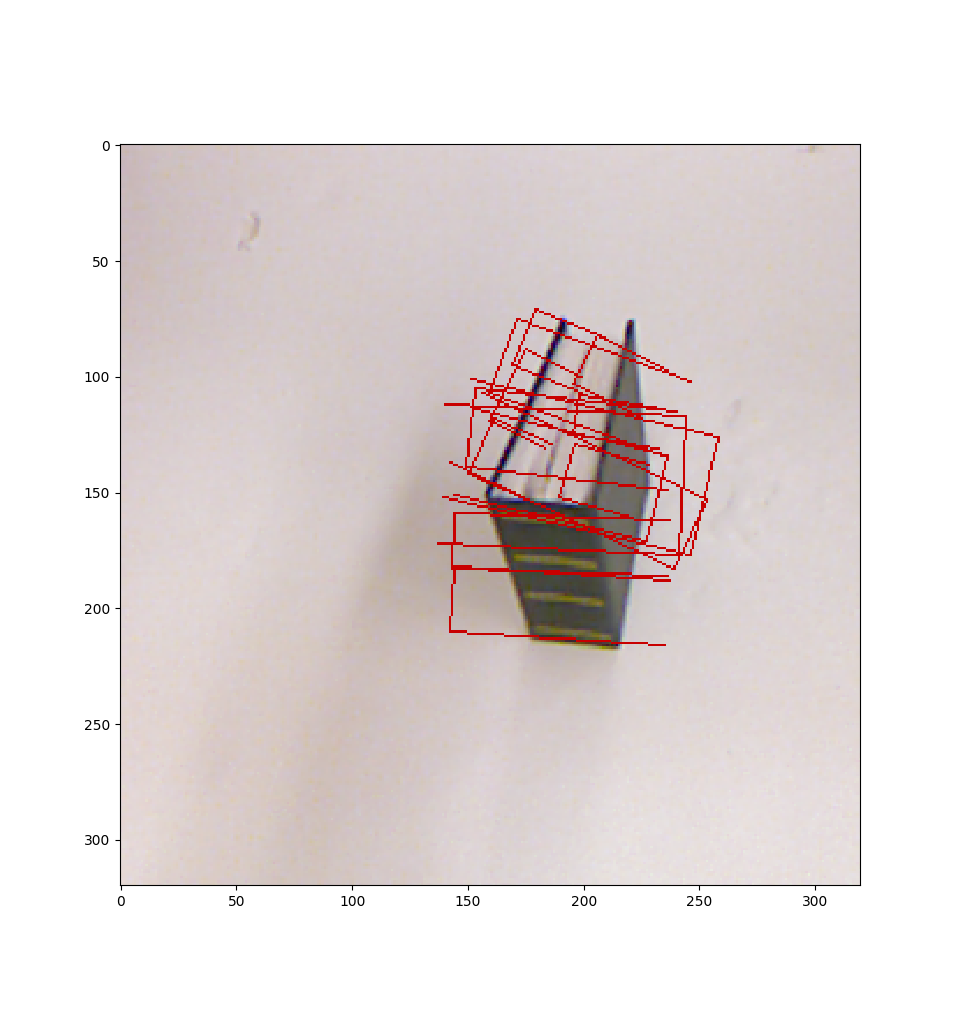
\includegraphics[width=0.3\textwidth]{figures/label_object_norm_1.png}}
\subfloat{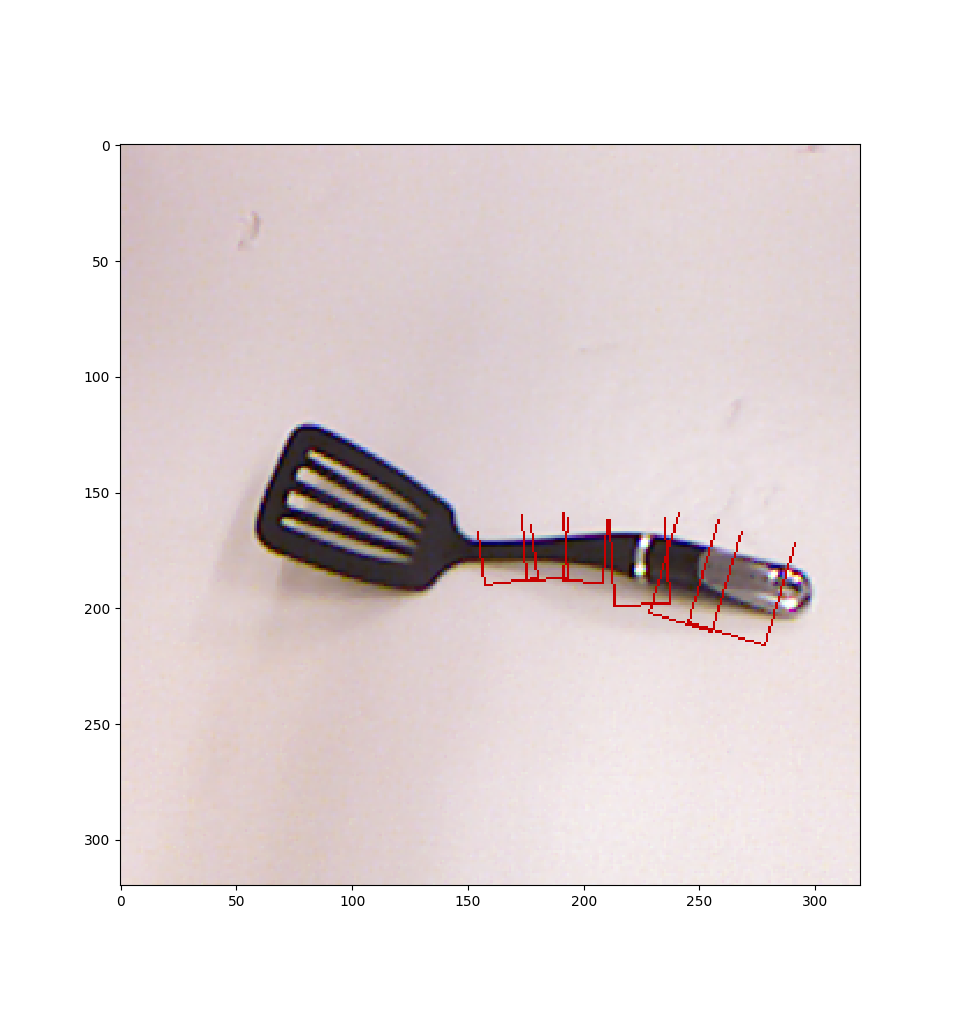
\includegraphics[width=0.3\textwidth]{figures/label_object_norm_2.png}}
\subfloat{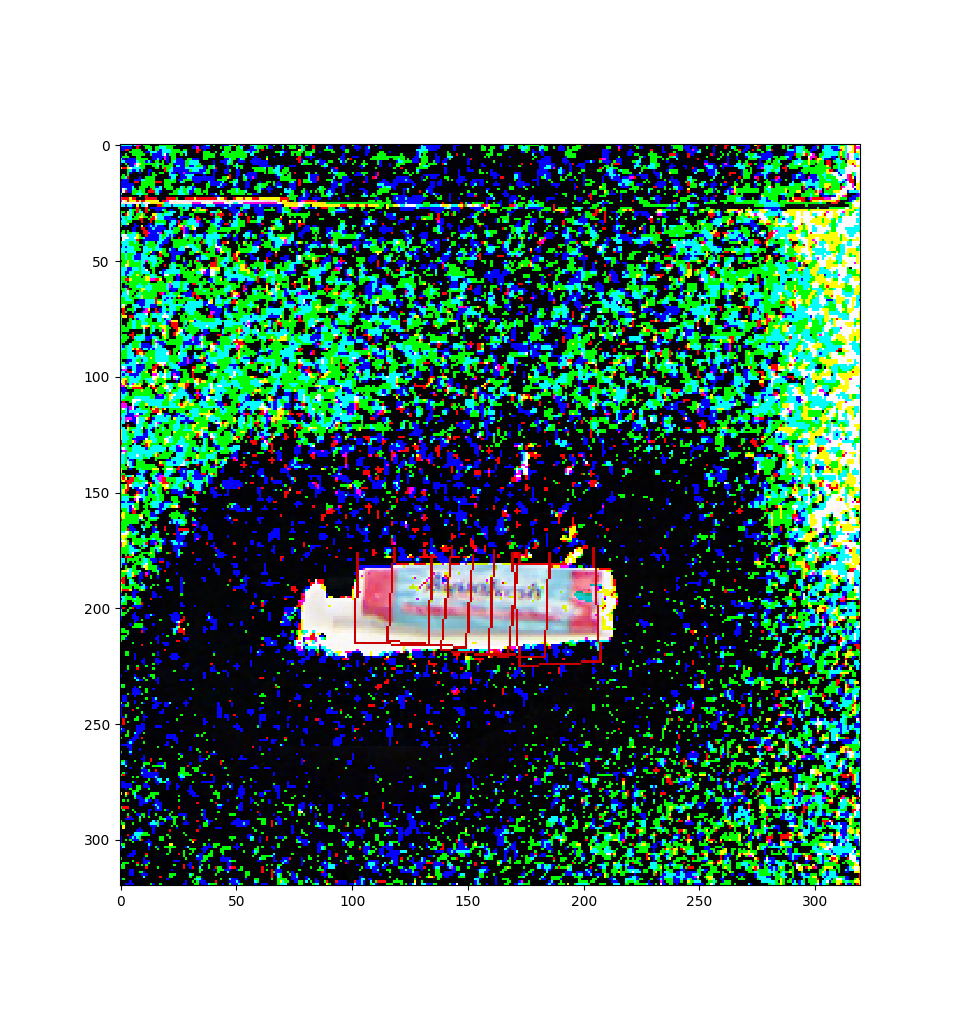
\includegraphics[width=0.3\textwidth]{figures/label_object_norm_3.png}}
\caption{Labeled images in the dataset, the right most image has background subtraction}
\end{figure}

\begin{figure}
\centering
\subfloat[Train]{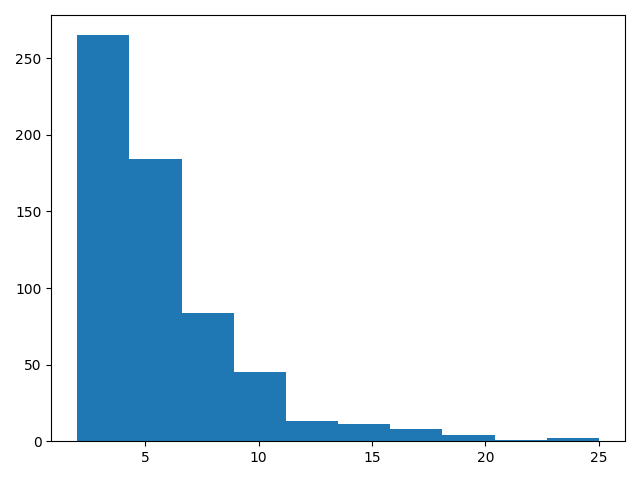
\includegraphics[width=0.4\textwidth]{figures/trainrecdist.png}}
\qquad
\subfloat[Val]{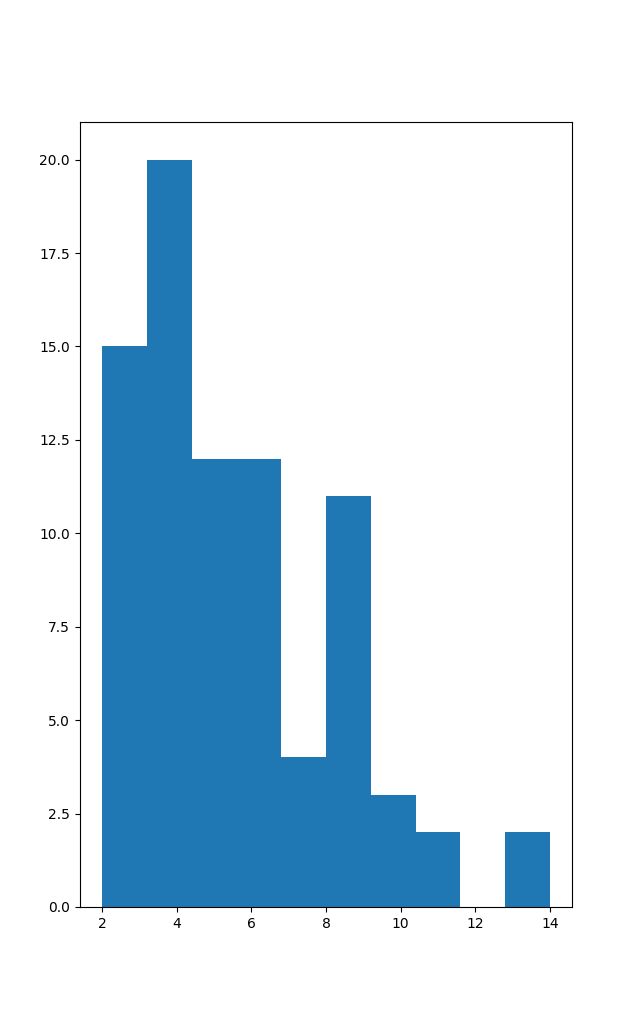
\includegraphics[width=0.4\textwidth]{figures/valrecdist.png}}
\caption{The Distribution of Rectangles per Image on the Training and Validation Sets}
\label{fig:recdist}
\end{figure}

The method used in this paper employs an anchor box
based detection model, so selecting the appropriate anchor box width is important.
Here we choose about 16 pixel width squares, as this results in few grasping
rectangles being connected to the same anchor box and having the largest anchor
size simultaneously. Avoiding overlapping anchor boxes is important because
during the training phase, as they introduce ambiguity.
See Figure \ref{fig:overlapdist} for a distribution of the number
of overlapping rectangles per image, given that anchor size is 16.

\begin{figure}
\centering
\subfloat[Train]{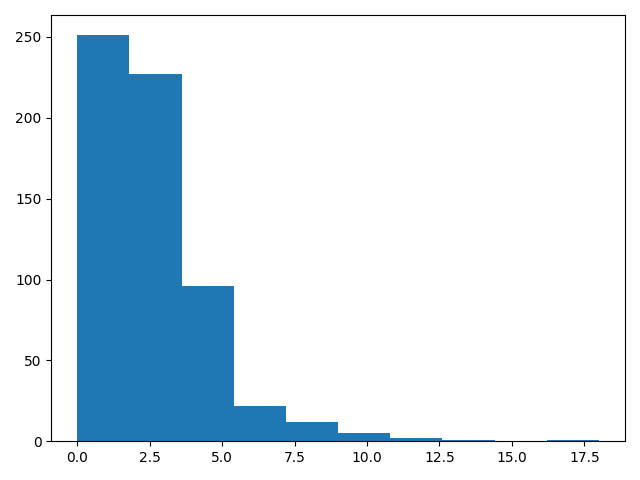
\includegraphics[width=0.4\textwidth]{figures/rec_overlaps_train.png}}
\qquad
\subfloat[Val]{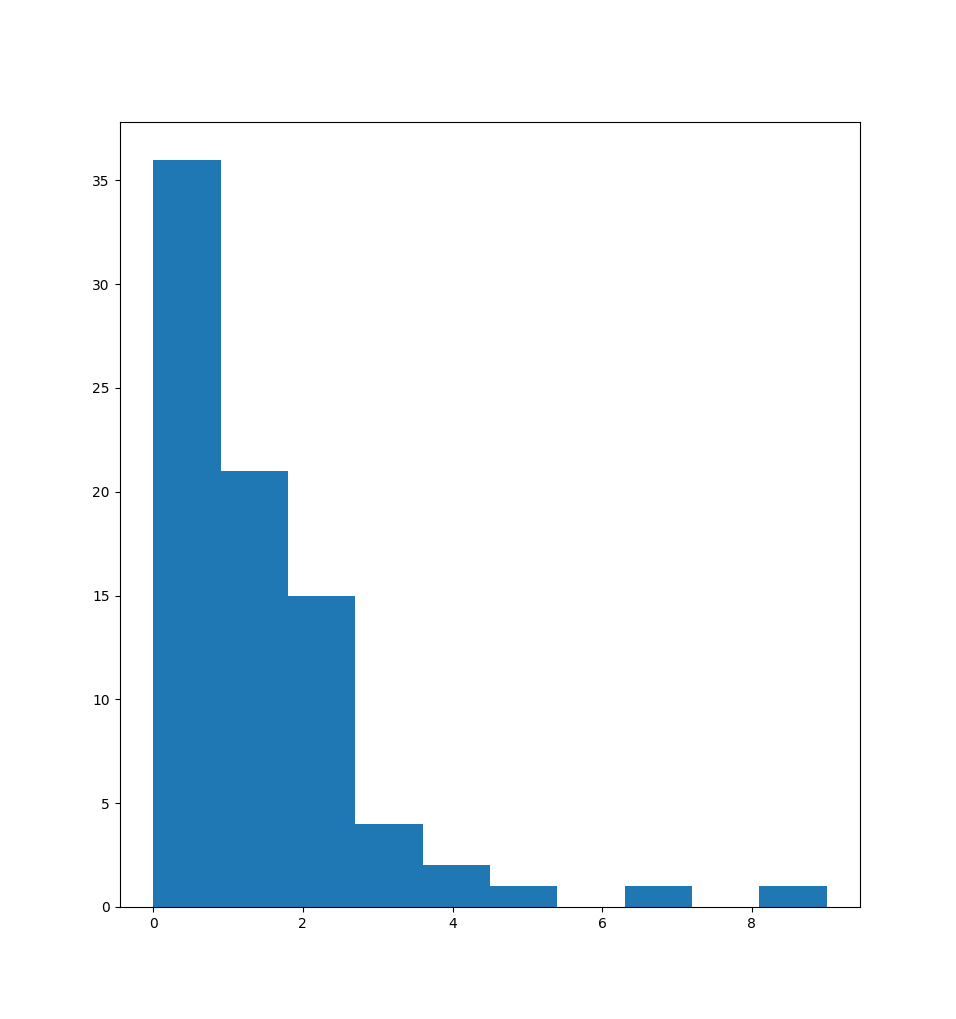
\includegraphics[width=0.4\textwidth]{figures/rec_overlaps_val.png}}
\caption{The Distribution of Number of Overlaps per Image on the Training and Validation Sets}
\label{fig:overlapdist}
\end{figure}

See Figure \ref{fig:summary} for detailed information about general
information of the dataset.

\begin{wrapfigure}{R}{0.5\textwidth}
\centering
\begin{tabular}{c|c|c|c|}
&Object&Images&Rectangles\\
\hline
Train&168&617&3567\\
\hline
Val&24&81&456\\
\hline
Test&52&185&1082\\
\hline
Totals&244&883&5105\\
\hline
\end{tabular}
\caption{Summary Counts of the Dataset}
\label{fig:summary}
\end{wrapfigure}


\subsection{Data Preprocessing}
Given that the dataset is small, in comparison with other datasets for deep
learning, it is important to perform data augmentation to prevent overfitting.
Following Zhang \textit{et al.} \cite{zhang18} the augmentation done to each
image is the following, a random flip horizontally, a random flip vertically,
a random rotation of the image about the center ranging from $-30\degree$ to
$30\degree$. The background image is also subtracted to reduce noise.

Every image also has a point cloud file, that contains depth data from a kinect
sensor. This is processed into an array and used as either separate input or
concatenated with the existing image tensor. Extracting the depth is written as an
extension of numpy, and can be found online in \textit{extract\_depth}.

I ran a series of tests, examining the input and targets as I change the task.
I take a look at how I could apply linear regression to the task and see if
I can get any results. I look at the depth data and see how I can extract
features from it. I look at how data augmentation affects the task, and the
clamping as well.

\section{Experiments}
I talk about the hardware I have access too. I trained some networks. I try
to run some ablation experiments with and without features I extracted (and
modification) in data analysis.

\bibliographystyle{plain}
\bibliography{bibliography.bib}

\end{document}
